\documentclass[10pt,a4paper]{article}
\usepackage[margin=2.1cm]{geometry}
\usepackage[T1]{fontenc}
\usepackage{mathptmx}
\usepackage[scaled=0.92]{helvet}
\usepackage{courier}
\usepackage[strings]{underscore}
\usepackage{microtype}
\usepackage{graphicx}
\usepackage{booktabs}
\usepackage{tabularx}
\usepackage{caption}
\usepackage{xcolor}
\usepackage{enumitem}
\usepackage[hidelinks]{hyperref}
\setlist{nosep,leftmargin=1.3em}
\captionsetup{font=small,labelfont=bf}
\newcommand{\AllocSpearman}{0.54}
\newcommand{\AllocSpearmanWO}{0.75}
\newcommand{\AllocsBzip}{0.0}
\newcommand{\AllocsGnugo}{0.0}
\newcommand{\AllocsHmmer}{0.0}
\newcommand{\AllocsLibxml}{4.7}
\newcommand{\AllocsLua}{10.7}
\newcommand{\AllocsLulesh}{0.0}
\newcommand{\AllocsPerl}{3.0}
\newcommand{\AllocsSqlite}{0.3}
\newcommand{\AllocsStockfish}{0.0}
\newcommand{\AllocsTrampd}{1.8}
\newcommand{\AllocsX}{0.0}
\newcommand{\BinAvg}{7.1}
\newcommand{\BinMax}{25.0}
\newcommand{\BinMin}{1.0}
\newcommand{\CodeAvg}{2.8}
\newcommand{\CodeMax}{3.4}
\newcommand{\CodeMin}{2.0}
\newcommand{\CtrlAsan}{2.06}
\newcommand{\CtrlDefBzip}{1.55}
\newcommand{\CtrlDefDelta}{0.31}
\newcommand{\CtrlDefGnugo}{2.06}
\newcommand{\CtrlDefHmmer}{1.64}
\newcommand{\CtrlDefLibxml}{2.16}
\newcommand{\CtrlDefLua}{3.60}
\newcommand{\CtrlDefLulesh}{1.59}
\newcommand{\CtrlDefPerl}{3.87}
\newcommand{\CtrlDefSqlite}{2.52}
\newcommand{\CtrlDefStockfish}{2.37}
\newcommand{\CtrlDefTrampd}{2.45}
\newcommand{\CtrlDefX}{2.31}
\newcommand{\CtrlDefault}{2.37}
\newcommand{\CtrlLean}{1.95}
\newcommand{\CtrlLeanDelta}{0.11}
\newcommand{\CtrlMemDefBzip}{1.77}
\newcommand{\CtrlMemDefGnugo}{4.29}
\newcommand{\CtrlMemDefHmmer}{5.05}
\newcommand{\CtrlMemDefLibxml}{2.30}
\newcommand{\CtrlMemDefLua}{13.62}
\newcommand{\CtrlMemDefLulesh}{13.87}
\newcommand{\CtrlMemDefMax}{21.3}
\newcommand{\CtrlMemDefMaxName}{tramp3d}
\newcommand{\CtrlMemDefPerl}{5.37}
\newcommand{\CtrlMemDefSqlite}{7.10}
\newcommand{\CtrlMemDefStockfish}{1.36}
\newcommand{\CtrlMemDefTrampd}{21.28}
\newcommand{\CtrlMemDefX}{1.76}
\newcommand{\CtrlMemDefault}{3.96}
\newcommand{\CtrlMemPaper}{1.47}
\newcommand{\CtrlPapBzip}{1.60}
\newcommand{\CtrlPapGnugo}{1.80}
\newcommand{\CtrlPapHmmer}{1.74}
\newcommand{\CtrlPapLibxml}{1.94}
\newcommand{\CtrlPapLua}{2.55}
\newcommand{\CtrlPapLulesh}{1.49}
\newcommand{\CtrlPapPerl}{2.60}
\newcommand{\CtrlPapSqlite}{2.19}
\newcommand{\CtrlPapStockfish}{2.08}
\newcommand{\CtrlPapTrampd}{2.01}
\newcommand{\CtrlPapX}{2.65}
\newcommand{\CtrlRuns}{5}
\newcommand{\GapMem}{-1.90}
\newcommand{\GapMemRel}{-56\%}
\newcommand{\GapPerl}{+0.22}
\newcommand{\GapPerlRel}{+8\%}
\newcommand{\GapRWAll}{+0.27}
\newcommand{\GapRWAllRel}{+16\%}
\newcommand{\GapRWMap}{+0.03}
\newcommand{\GapRWMapRel}{+1\%}
\newcommand{\GapWOAll}{+0.19}
\newcommand{\GapWOAllRel}{+15\%}
\newcommand{\GapWOMap}{-0.03}
\newcommand{\GapWOMapRel}{-2\%}
\newcommand{\GapXml}{-0.75}
\newcommand{\GapXmlRel}{-28\%}
\newcommand{\MainRuns}{15}
\newcommand{\MaxBaseCV}{25.3}
\newcommand{\MaxRWsd}{0.62}
\newcommand{\MedBaseCV}{18}
\newcommand{\MedianAvgRW}{2.01}
\newcommand{\MedianAvgWO}{1.47}
\newcommand{\MemAddBzip}{4}
\newcommand{\MemAddGnugo}{14}
\newcommand{\MemAddHmmer}{7}
\newcommand{\MemAddLibxml}{345}
\newcommand{\MemAddLua}{46}
\newcommand{\MemAddLulesh}{9}
\newcommand{\MemAddPerl}{24}
\newcommand{\MemAddSqlite}{52}
\newcommand{\MemAddStockfish}{7}
\newcommand{\MemAddTrampd}{7}
\newcommand{\MemAddX}{10}
\newcommand{\MemBzip}{1.46}
\newcommand{\MemGnugo}{1.63}
\newcommand{\MemHmmer}{2.43}
\newcommand{\MemLibxml}{1.65}
\newcommand{\MemLua}{1.92}
\newcommand{\MemLulesh}{1.39}
\newcommand{\MemPerl}{1.23}
\newcommand{\MemSqlite}{1.56}
\newcommand{\MemStockfish}{1.03}
\newcommand{\MemTrampd}{1.32}
\newcommand{\MemX}{1.34}
\newcommand{\MinName}{bzip2}
\newcommand{\MinVal}{1.48}
\newcommand{\NnueMB}{69}
\newcommand{\NumHiAlloc}{4}
\newcommand{\OurAvgRW}{2.00}
\newcommand{\OurAvgRWpct}{100}
\newcommand{\OurAvgRWsd}{0.05}
\newcommand{\OurAvgWO}{1.45}
\newcommand{\OurAvgWOpct}{45}
\newcommand{\OurAvgWOsd}{0.05}
\newcommand{\OurGeoRW}{1.94}
\newcommand{\OurGeoWO}{1.40}
\newcommand{\OurMapRW}{1.98}
\newcommand{\OurMapRWsd}{0.11}
\newcommand{\OurMapWO}{1.43}
\newcommand{\OurMapWOsd}{0.06}
\newcommand{\OurMemAvg}{1.54}
\newcommand{\OurMemAvgsd}{0.01}
\newcommand{\OurMemMapTotal}{1.45}
\newcommand{\OurMemTotal}{1.47}
\newcommand{\OurMemWOTotal}{1.47}
\newcommand{\PaperMapRW}{1.95}
\newcommand{\PaperMapWO}{1.46}
\newcommand{\PaperMemMapTotal}{3.11}
\newcommand{\PaperWOShare}{36}
\newcommand{\RWBzip}{1.48}
\newcommand{\RWGnugo}{1.53}
\newcommand{\RWHmmer}{1.56}
\newcommand{\RWLibxml}{1.92}
\newcommand{\RWLua}{2.47}
\newcommand{\RWLulesh}{1.56}
\newcommand{\RWPerl}{2.82}
\newcommand{\RWSqlite}{1.98}
\newcommand{\RWStockfish}{2.33}
\newcommand{\RWTrampd}{2.14}
\newcommand{\RWX}{2.22}
\newcommand{\RWsdBzip}{0.27}
\newcommand{\RWsdGnugo}{0.17}
\newcommand{\RWsdHmmer}{0.16}
\newcommand{\RWsdLibxml}{0.25}
\newcommand{\RWsdLua}{0.62}
\newcommand{\RWsdLulesh}{0.23}
\newcommand{\RWsdPerl}{0.27}
\newcommand{\RWsdSqlite}{0.26}
\newcommand{\RWsdStockfish}{0.26}
\newcommand{\RWsdTrampd}{0.31}
\newcommand{\RWsdX}{0.40}
\newcommand{\RuntimeKB}{1256}
\newcommand{\RzMemFlat}{7}
\newcommand{\RzMemMostName}{lua}
\newcommand{\RzMemMostsixteen}{1.77}
\newcommand{\RzMemMosttwofiftysix}{5.55}
\newcommand{\RzMemSpearman}{0.65}
\newcommand{\RzMonetwentyeight}{1.93}
\newcommand{\RzMostName}{lua}
\newcommand{\RzMostTsixteen}{2.54}
\newcommand{\RzMostTtwofiftysix}{3.65}
\newcommand{\RzMsixteen}{1.45}
\newcommand{\RzMsixtyfour}{1.55}
\newcommand{\RzMthirtytwo}{1.47}
\newcommand{\RzMtwofiftysix}{2.71}
\newcommand{\RzRuns}{5}
\newcommand{\RzSpearman}{0.35}
\newcommand{\RzTonetwentyeight}{2.14}
\newcommand{\RzTonetwentyeightsd}{0.19}
\newcommand{\RzTsixteen}{2.03}
\newcommand{\RzTsixteensd}{0.10}
\newcommand{\RzTsixtyfour}{2.13}
\newcommand{\RzTsixtyfoursd}{0.11}
\newcommand{\RzTthirtytwo}{2.11}
\newcommand{\RzTthirtytwosd}{0.19}
\newcommand{\RzTtwofiftysix}{2.20}
\newcommand{\RzTtwofiftysixsd}{0.11}
\newcommand{\StackNoticeable}{1}
\newcommand{\StackOverTen}{1}
\newcommand{\StealAdjMeanSD}{0.07}
\newcommand{\StealAdjRW}{2.00}
\newcommand{\StealAdjRWsd}{0.02}
\newcommand{\StealAdjWO}{1.46}
\newcommand{\StealCVadj}{4}
\newcommand{\StealCVraw}{15}
\newcommand{\StealMaxPct}{48}
\newcommand{\StealPct}{9}
\newcommand{\StealRawMeanSD}{0.29}
\newcommand{\StealRawRW}{2.01}
\newcommand{\StealRuns}{10}
\newcommand{\TopOne}{2.82}
\newcommand{\TopOneName}{perl}
\newcommand{\TopTwo}{2.47}
\newcommand{\TopTwoName}{lua}
\newcommand{\VmPeakAsanTB}{20.0}
\newcommand{\VmPeakAsanTBmax}{20.0}
\newcommand{\WOBzip}{1.10}
\newcommand{\WOGnugo}{1.19}
\newcommand{\WOHmmer}{1.10}
\newcommand{\WOLibxml}{1.78}
\newcommand{\WOLua}{2.06}
\newcommand{\WOLulesh}{1.11}
\newcommand{\WOPerl}{2.18}
\newcommand{\WOShare}{45}
\newcommand{\WOShareHi}{63}
\newcommand{\WOShareLo}{28}
\newcommand{\WOSqlite}{1.47}
\newcommand{\WOStockfish}{1.39}
\newcommand{\WOTrampd}{1.34}
\newcommand{\WOX}{1.27}

\newcommand{\asan}{ASan}
\newcommand{\cmd}[1]{\texttt{#1}}

\title{\textbf{Reproducing ``AddressSanitizer: A Fast Address Sanity Checker''}\\[2pt]
\large CS340 Operating Systems --- Research Paper Replication Report}
\author{Group 19:\;
Hua Minqi (1240030798),\; Li Linxuan (1240022141),\; You Te (1240037846)\\[2pt]
\small Repository: \url{https://github.com/CodeShiTianmin/AddressSanitizer} (tag \texttt{v1.0})}
\date{December 2026}

\begin{document}
\maketitle

\begin{abstract}
\noindent
AddressSanitizer (\asan{}) detects out-of-bounds accesses and use-after-free
bugs in C/C++ programs through compiler instrumentation and shadow memory.
The paper reports a 73\% average slowdown and a 3.37$\times$ memory increase on
SPEC CPU2006. We re-measured the performance evaluation (Section~4 of the
paper) with clang~18.1.3 on 11 open-source programs, seven of which are the
same program as, or the same kind of application as, a SPEC CPU2006 benchmark.
For these seven programs the average slowdown is
\OurMapRW$\pm$\OurMapRWsd$\times$, while their SPEC counterparts average
\PaperMapRW$\times$ in the paper. Instrumenting only writes gives
\OurMapWO$\times$ against \PaperMapWO$\times$. Over all 11 programs the
averages are \OurAvgRW$\times$ (reads and writes) and \OurAvgWO$\times$
(writes only), above the paper's 1.73$\times$ and 1.26$\times$; this gap
comes from the workload mix, since the paper's own values for our counterparts
are also above its average. Under the paper's settings
the memory increase is \OurMemTotal$\times$ in peak resident memory, much less
than 3.37$\times$; the paper's own metric (VmPeak) no longer works, because
current \asan{} reserves 20\,TB of virtual address space at start-up. Binaries
grow by \CodeMin--\CodeMax$\times$ once the statically linked run-time is
excluded, close to the paper's 1.5--3.2$\times$. As an extension we varied the
heap redzone size from 16 to 256 bytes. The total memory increase grows from
\RzMsixteen$\times$ to \RzMtwofiftysix$\times$, driven by the programs that keep
many small heap objects live, while the run time changes little except for the
two most allocation-intensive programs. This supports the paper's
unquantified remark in its Section~4.3 for memory, and only partly for time.
\end{abstract}

% ===========================================================================
\section{Introduction and Claims}\label{sec:intro}

\paragraph{Paper and problem.}
Memory-safety bugs in C and C++ (buffer overflows on the heap, the stack or in
globals, and use-after-free) are a major source of crashes and security
vulnerabilities. Before \asan{}, tools for finding them were either slow
(Valgrind's Memcheck and Dr.~Memory slow programs down by 10--20$\times$ on
SPEC~\cite{asan}) or found only some of these bugs (debug allocators with
guard pages). Serebryany et al.~\cite{asan} make the bugs detectable cheaply in
three ways:
\begin{enumerate}
\item every 8 bytes of application memory map to one byte of \emph{shadow
memory} (\cmd{Shadow = (Addr >> 3) + Offset}), which records how many of
those bytes may be accessed;
\item the compiler inserts a shadow check before every load and store;
\item a replacement allocator surrounds heap objects with poisoned
\emph{redzones} (the compiler does the same for stack and global objects) and
holds freed memory in a FIFO \emph{quarantine}.
\end{enumerate}
The checks run inline, so the overhead depends on how much a program accesses
memory and allocates, which is an OS-level concern (address-space layout,
virtual memory reservation, allocator design).

\paragraph{Claims tested.}
\begin{description}[leftmargin=0pt]
\item[C1 (Figure 2, \S4).] With reads and writes instrumented, \asan{} slows
SPEC CPU2006 down by 73\% on average (1.73$\times$). The malloc-intensive
text-processing benchmarks are slowed the most (perlbench 2.60$\times$,
xalancbmk 2.67$\times$).
\item[C2 (Figure 2, \S4).] With only writes instrumented, the average slowdown
drops to 26\%.
\item[C3 (Tables 1--2, \S4).] Memory use grows by 3.37$\times$, mostly
because of the malloc redzones. Only a few programs need noticeably more
stack. Binaries grow by 1.5--3.2$\times$ (2.5$\times$ on average).
\end{description}

\paragraph{Scope.}
We reproduce the performance evaluation of Section~4: run time (C1, C2),
memory, stack and binary size (C3). We use 11 open-source programs whose base
runs take 2--4\,s, instead of the 19 C/C++ SPEC CPU2006 benchmarks with
reference inputs. We add controlled re-runs that separate changes made to
\asan{} since 2012 (\S\ref{sec:analysis}), and one extension, a sweep of the
heap redzone size (\S\ref{sec:ext}). We do not reproduce:
\begin{itemize}
\item the deployment statistics from Chromium (\S4.2);
\item the measurements of other tools (\S4.1);
\item the experiment that varies the shadow \emph{Scale} and \emph{Offset}.
Current \asan{} fixes the shadow scale when its run-time library is built, so
this experiment would require a custom build of compiler-rt.
\end{itemize}

% ===========================================================================
\section{Reproduction Setup}\label{sec:setup}

\paragraph{Starting code.}
The paper has no separate artifact. \asan{} was merged into LLVM in 2011 and is
maintained there. We use the unmodified \asan{} of \textbf{clang 18.1.3}
(Ubuntu package \cmd{1:18.1.3-1ubuntu1}, upstream tag \cmd{llvmorg-18.1.3}).
Our repository contains only build scripts, workload drivers, a measurement
harness and analysis code. No source file of \asan{} or of the benchmarked
programs is modified; the repository's \cmd{README} lists the starting commit
and the files we wrote. The programs are downloaded from upstream and checked
against SHA-256 hashes (\cmd{scripts/sources.txt}).

\paragraph{Environment.}
Builds and runs happen inside a Docker image. Its \cmd{ubuntu:24.04} base is
pinned by digest and clang by package version (\cmd{Dockerfile}).
Table~\ref{tab:env} compares our machine with the paper's.

\begin{table}[t]
\centering\small
\caption{Environment of the paper and of our runs (ours recorded in \cmd{results/env.txt}).}\label{tab:env}
\begin{tabularx}{\linewidth}{lXX}
\toprule
Item & Paper~\cite{asan} & Ours \\
\midrule
Machine & HP Z600, 2$\times$ quad-core Xeon E5620, 24\,GB & KVM virtual machine, Intel Xeon (family 6, model 94), 2 vCPU, 8\,GB \\
OS / kernel & 64-bit Linux (version not stated) & Ubuntu 24.04 container on Ubuntu 22.04, Linux 6.8.0-1060-aws \\
Compiler & LLVM/clang of early 2012 (version not stated) & clang 18.1.3, glibc 2.39 \\
Baseline & \cmd{clang -O2} & \cmd{clang -O2} \\
Workloads & SPEC CPU2006, 19 C/C++ benchmarks, ref.\ inputs & 11 open-source programs (Table~\ref{tab:workloads}) \\
Repetitions & not stated & \MainRuns{} (main), \CtrlRuns{} (controls), \RzRuns{} (extension), interleaved \\
Pinning / ASLR & not stated & \cmd{taskset} to one vCPU; ASLR on (default) \\
\bottomrule
\end{tabularx}
\end{table}

\paragraph{Workloads.}
SPEC CPU2006 requires a licence that we do not have, so we chose open-source
programs that resemble the SPEC programs as closely as possible
(Table~\ref{tab:workloads}):
\begin{itemize}
\item four are newer releases of the same programs that SPEC packages
(\cmd{perl}, \cmd{bzip2}, \cmd{gnugo}, \cmd{hmmer});
\item three come from the same application domain as a SPEC benchmark: a chess
engine, an H.264 encoder and an XML processor;
\item two are C++ floating-point codes (\cmd{tramp3d}, \cmd{lulesh}), which we
compare to dealII and milc only loosely;
\item two have no SPEC counterpart (a Lua interpreter and SQLite).
\end{itemize}
The ``7 counterparts'' rows in our tables average over \cmd{perl},
\cmd{bzip2}, \cmd{gnugo}, \cmd{hmmer}, \cmd{stockfish}, \cmd{x264} and
\cmd{libxml2}. All inputs are generated deterministically
(\cmd{scripts/gen_inputs.py}, fixed seed) or taken from the pinned source
archives.

\begin{table}[t]
\centering\small
\caption{Workloads. Base run times are in Table~\ref{tab:time}.}\label{tab:workloads}
\begin{tabularx}{\linewidth}{lllX}
\toprule
Ours & Version & SPEC CPU2006 counterpart & Workload \\
\midrule
\cmd{perl} (miniperl) & 5.38.2 & 400.perlbench (same program) & regexes, hashes, sorting over 6\,MB of Perl source text \\
\cmd{bzip2} & 1.0.8 & 401.bzip2 (same program) & \cmd{-9} compress + decompress 24\,MB of mixed text/binary \\
\cmd{gnugo} & 3.8 & 445.gobmk (same program) & GTP self-play, 13$\times$13, 24 moves, level 8 \\
\cmd{hmmer} & 3.4 & 456.hmmer (same program) & \cmd{hmmbuild} (Pkinase) + \cmd{hmmsearch --max} over 8000 random proteins \\
\cmd{stockfish} & 16.1 & 458.sjeng (chess engine) & \cmd{bench 16 1 14} (1 thread, depth 14) \\
\cmd{x264} & 31e19f92 & 464.h264ref (H.264 encoder) & 150 CIF frames, preset medium, C code only (\cmd{--disable-asm}) \\
\cmd{libxml2} & 2.12.9 & 483.xalancbmk (XML processing) & \cmd{xmllint --format} + XPath query on 40\,MB XML \\
\cmd{tramp3d} & test-suite 18.1.8 & (447.dealII, C++ templates) & \cmd{-n 100 --domain 40 40 40} \\
\cmd{lulesh} & 2.0.3 & (433.milc, FP physics) & \cmd{-s 30 -i 150}, serial \\
\cmd{lua} & 5.4.6 & -- (interpreter) & binary-trees, fannkuch, string building, spectral-norm \\
\cmd{sqlite} & 3.46.0 & -- (database) & \cmd{speedtest1 --memdb --size 120} \\
\bottomrule
\end{tabularx}
\end{table}

\paragraph{Configurations and measurement.}
Every program is built with its own build system in the four
configurations defined in \cmd{config/build_configs.sh}:
\begin{itemize}
\item \cmd{base}: \cmd{-O2}.
\item \cmd{asan}: \cmd{-O2 -fsanitize=address}.
\item \cmd{asanwo}: additionally \cmd{-mllvm -asan-instrument-reads=false},
so only writes are checked.
\item \cmd{asanlean}: a control build without two instrumentation features
added after 2012, stack-use-after-return support and use-after-scope
poisoning.
\end{itemize}
The paper's run-time settings are used unless stated otherwise (\S4 of the
paper; \cmd{config/experiments.json}): \cmd{redzone=32},
\cmd{malloc\_context\_size=0} (no stack unwinding in malloc/free),
\cmd{quarantine\_size\_mb=0}, and \cmd{detect\_leaks=0} and
\cmd{detect\_stack\_use\_after\_return=0} for two features that did not exist
in 2012.

The harness (\cmd{scripts/run_experiments.py}) works as follows:
\begin{itemize}
\item every run is pinned to one vCPU, and one unrecorded warm-up run is made
per program;
\item within each repetition, every program runs once in every variant, and
the order of the variants rotates from one repetition to the next;
\item we record wall-clock time and, at exit of every process, the
\cmd{VmPeak}, \cmd{VmHWM} (peak resident set) and \cmd{VmStk} fields of
\cmd{/proc/self/status}, via a small \cmd{LD\_PRELOAD} library
(\cmd{harness/procstat.c}). The paper used the same method;
\item a slowdown is the variant's time divided by the base time of the same
repetition. We report mean~$\pm$~sample standard deviation over repetitions;
\item averages over programs are arithmetic means, like the paper's
``average'' bar: the mean of the 19 bars we digitized from Figure~2 is 1.74,
against the stated 1.73;
\item a second \cmd{LD\_PRELOAD} library (\cmd{harness/malloccount.c}) counts
heap allocations in the base builds.
\end{itemize}
Each run appends one JSON record to \cmd{results/raw/<experiment>/runs.jsonl}.
All tables, figures and numbers in this report are produced from those records
by \cmd{analysis/analyze.py}.

\paragraph{Deviations.}
Table~\ref{tab:dev} lists every difference from the paper's setup.

\begin{table}[t]
\centering\small
\caption{Deviations from the paper's setup.}\label{tab:dev}
\begin{tabularx}{\linewidth}{lXXX}
\toprule
Item & Paper & Ours & Reason \\
\midrule
Benchmarks & 19 SPEC CPU2006 C/C++ & 11 open-source programs, 7 with a SPEC counterpart & SPEC licence not available \\
Input size & SPEC reference inputs (minutes) & 2--4\,s per base run & 2-vCPU VM; $\geq$5 repetitions of up to 6 variants \\
Compiler & clang, early 2012 & clang 18.1.3 & the 2012 tool is not stated precisely and does not build with current toolchains; we test whether the claims still hold \\
Hardware & 8-core Westmere workstation, 24\,GB & 2-vCPU KVM VM, 8\,GB & machine available to us \\
Redzone & 32\,B & \cmd{redzone=32} is now a \emph{minimum}; larger chunks get larger redzones & option semantics changed \\
Newer features & not present & leak checking and stack-use-after-return off at run time; use-after-scope and UAR hooks still compiled in & isolated by the \cmd{asanlean} control (\S\ref{sec:analysis}) \\
Memory metric & VmPeak & VmHWM (peak RSS); VmPeak also recorded & \asan{} now reserves $\approx$20\,TB of virtual shadow memory, so VmPeak is $\approx$20\,TB for every program \\
Writes-only mode & flag not stated & \cmd{-mllvm} \cmd{-asan-instrument-\allowbreak{}reads=false} & current equivalent \\
Multi-process runs & single process & \cmd{bzip2}, \cmd{hmmer}, \cmd{libxml2} run two commands; time summed, memory = maximum over processes & SPEC-like input sets \\
Perl & full perl, static & \cmd{miniperl} (no dynamic loading) & avoids loading instrumented shared objects; same interpreter core \\
Scale/Offset study & Scale 3--7, Offset 0 & not reproduced & shadow scale is fixed when the run-time is built \\
\bottomrule
\end{tabularx}
\end{table}

% ===========================================================================
\section{Results}\label{sec:results}

\paragraph{Run time (C1, C2).}
Table~\ref{tab:time} and Figure~\ref{fig:slowdown} compare our slowdowns with
the paper's. Over all 11 programs \asan{} slows execution down by
\OurAvgRW$\pm$\OurAvgRWsd$\times$ (\OurAvgRWpct\%; geometric mean
\OurGeoRW$\times$). Checking only writes gives
\OurAvgWO$\pm$\OurAvgWOsd$\times$ (\OurAvgWOpct\%). For the seven programs
with a SPEC counterpart, the averages are \OurMapRW$\pm$\OurMapRWsd$\times$
and \OurMapWO$\pm$\OurMapWOsd$\times$; the paper's values for the same seven
SPEC benchmarks are \PaperMapRW$\times$ and \PaperMapWO$\times$. The largest
slowdowns are for \cmd{\TopOneName} (\TopOne$\times$) and \cmd{\TopTwoName}
(\TopTwo$\times$), and the smallest for \cmd{\MinName} (\MinVal$\times$).

\begin{table}[t]
\centering\small
\caption{Paper vs.\ Ours: slowdown relative to \cmd{clang -O2} (mean $\pm$
s.d.\ over \MainRuns{} runs). ``Paper'' columns are read from Figure~2
($\pm$0.03), except the exact values given in the text (perlbench 2.60,
xalancbmk 2.67, averages 1.73/1.26). R+W = reads and writes instrumented,
W = writes only. Raw data: \cmd{results/raw/main/runs.jsonl}.}\label{tab:time}
\begin{tabular}{llrrrrr}
\toprule
Ours & SPEC counterpart & Base [s] & Paper R+W & Ours R+W & Paper W & Ours W \\
\midrule
\texttt{perl} & 400.perlbench & 2.88 & 2.60 & 2.82$\pm$0.27 & 2.19 & 2.18$\pm$0.35 \\
\texttt{bzip2} & 401.bzip2 & 2.86 & 1.83 & 1.48$\pm$0.27 & 1.26 & 1.10$\pm$0.18 \\
\texttt{gnugo} & 445.gobmk & 2.50 & 1.69 & 1.53$\pm$0.17 & 1.22 & 1.19$\pm$0.18 \\
\texttt{hmmer} & 456.hmmer & 3.83 & 1.80 & 1.56$\pm$0.16 & 1.25 & 1.10$\pm$0.13 \\
\texttt{stockfish} & 458.sjeng & 2.33 & 1.60 & 2.33$\pm$0.26 & 1.24 & 1.39$\pm$0.21 \\
\texttt{x264} & 464.h264ref & 3.11 & 1.46 & 2.22$\pm$0.40 & 1.20 & 1.27$\pm$0.13 \\
\texttt{libxml2} & 483.xalancbmk & 2.47 & 2.67 & 1.92$\pm$0.25 & 1.85 & 1.78$\pm$0.27 \\
\texttt{tramp3d} & 447.dealII & 2.11 & 2.04 & 2.14$\pm$0.31 & 1.42 & 1.34$\pm$0.18 \\
\texttt{lulesh} & 433.milc & 2.53 & 1.50 & 1.56$\pm$0.23 & 1.17 & 1.11$\pm$0.05 \\
\texttt{lua} & -- & 2.87 & -- & 2.47$\pm$0.62 & -- & 2.06$\pm$0.28 \\
\texttt{sqlite} & -- & 2.60 & -- & 1.98$\pm$0.26 & -- & 1.47$\pm$0.22 \\
\midrule
Average (7 counterparts) &  &  & 1.95 & 1.98$\pm$0.11 & 1.46 & 1.43$\pm$0.06 \\
Average (all 11) & SPEC avg. &  & 1.73 & 2.00$\pm$0.05 & 1.26 & 1.45$\pm$0.05 \\
Geometric mean (all 11) &  &  & 1.70 & 1.94$\pm$0.05 & 1.25 & 1.40$\pm$0.05 \\
\bottomrule
\end{tabular}

\end{table}

\begin{figure}[t]
\centering
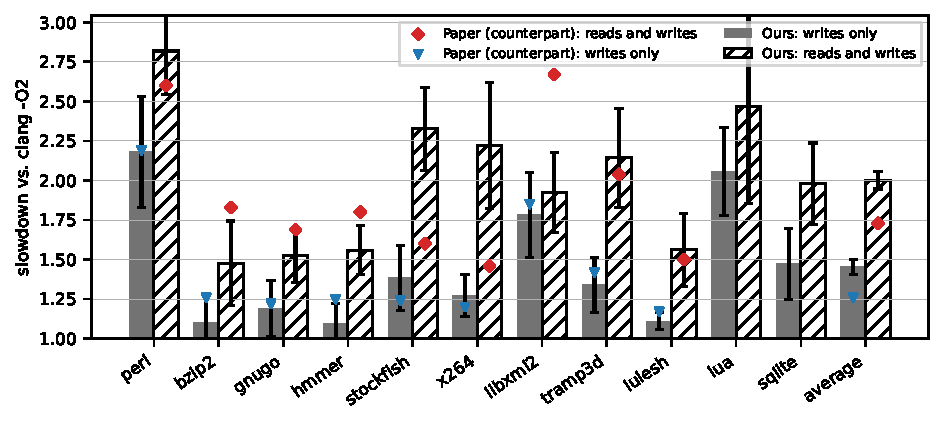
\includegraphics[width=\linewidth]{figures/fig_slowdown.pdf}
\caption{Our slowdowns in the style of the paper's Figure~2 (error bars: s.d.\
over \MainRuns{} runs). Markers show the paper's values for the SPEC
counterpart of each program.}\label{fig:slowdown}
\end{figure}

\paragraph{Memory, stack and binary size (C3).}
Table~\ref{tab:mem} and Figure~\ref{fig:mem} show peak memory. Summed over
all programs, as in the ``total'' row of the paper's Table~1, peak resident
memory grows by \OurMemTotal$\times$ (\OurMemMapTotal$\times$ for the seven
counterparts, whose SPEC versions grow by \PaperMemMapTotal$\times$ in the
paper). The mean of the per-program ratios is
\OurMemAvg$\pm$\OurMemAvgsd$\times$. Every \asan{} process has a VmPeak of
\VmPeakAsanTB\,TB. Stack size (Table~\ref{tab:stack}) changes by more than 5\%
for \StackNoticeable{} of the 11 programs. The program code itself (excluding
the \RuntimeKB\,KB statically linked \asan{} run-time) grows by
\CodeMin--\CodeMax$\times$, \CodeAvg$\times$ on average
(Table~\ref{tab:bin}); the paper reports 1.5--3.2$\times$, 2.5$\times$ on
average.

\begin{table}[t]
\centering\small
\caption{Paper vs.\ Ours: peak memory in MB (VmHWM, mean over \MainRuns{}
runs) and VmPeak, \asan{} with the paper's settings. ``Paper incr.'' is the
Table~1 ratio (VmPeak) of the SPEC counterpart. Raw data:
\cmd{results/raw/main/runs.jsonl}, field \cmd{procs}.}\label{tab:mem}
\begin{tabular}{lrrrrrr}
\toprule
Benchmark & Base RSS & ASan RSS & Ours incr. & Paper incr. & Base VmPeak & ASan VmPeak \\
\midrule
\texttt{perl} & 103 & 127 & 1.23$\pm$0.00 & 3.24 & 106 & 20.0 TB \\
\texttt{bzip2} & 9 & 13 & 1.46$\pm$0.01 & 1.89 & 10 & 20.0 TB \\
\texttt{gnugo} & 22 & 35 & 1.63$\pm$0.01 & 9.97 & 26 & 20.0 TB \\
\texttt{hmmer} & 5 & 12 & 2.43$\pm$0.03 & 17.64 & 6 & 20.0 TB \\
\texttt{stockfish} & 217 & 224 & 1.03$\pm$0.00 & 1.38 & 305 & 20.0 TB \\
\texttt{x264} & 28 & 38 & 1.34$\pm$0.00 & 6.10 & 33 & 20.0 TB \\
\texttt{libxml2} & 534 & 879 & 1.65$\pm$0.00 & 3.89 & 556 & 20.0 TB \\
\texttt{tramp3d} & 21 & 28 & 1.32$\pm$0.01 & 3.22 & 24 & 20.0 TB \\
\texttt{lulesh} & 23 & 33 & 1.39$\pm$0.01 & 2.33 & 26 & 20.0 TB \\
\texttt{lua} & 50 & 97 & 1.92$\pm$0.09 & -- & 52 & 20.0 TB \\
\texttt{sqlite} & 92 & 143 & 1.56$\pm$0.00 & -- & 93 & 20.0 TB \\
\midrule
Total (7 counterparts) & 918 & 1328 & 1.45 & 3.11 &  &  \\
Total (all 11) & 1105 & 1629 & 1.47 & 3.37 &  &  \\
Mean of ratios &  &  & 1.54$\pm$0.01 &  &  &  \\
\bottomrule
\end{tabular}

\end{table}

\begin{figure}[t]
\centering
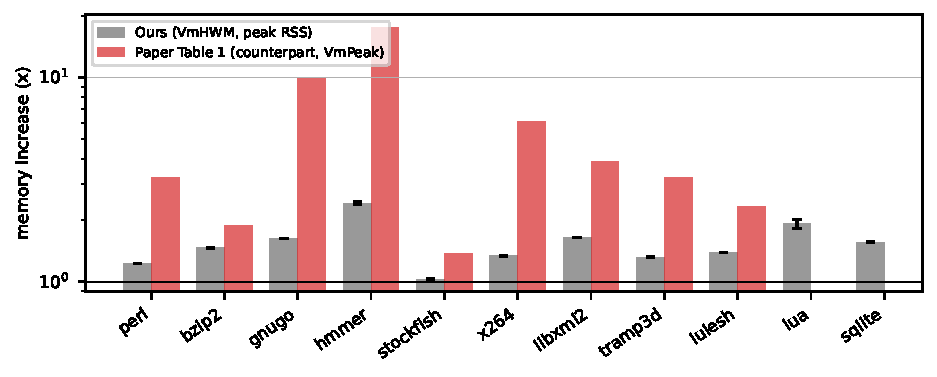
\includegraphics[width=\linewidth]{figures/fig_memory.pdf}
\caption{Memory increase: ours (peak RSS, error bars: s.d.) vs.\ paper
Table~1 (VmPeak) for the SPEC counterpart. Log scale.}\label{fig:mem}
\end{figure}

\begin{table}[t]
\centering\small
\caption{Stack (VmStk at exit, KB, mean). Paper: Table~2.}\label{tab:stack}
\begin{tabular}{lrrrr}
\toprule
Benchmark & Base VmStk [KB] & ASan VmStk [KB] & Increase & Paper (counterpart) \\
\midrule
\texttt{perl} & 132 & 132 & 1.00x & 3.06x \\
\texttt{bzip2} & 132 & 132 & 1.00x & -- \\
\texttt{gnugo} & 217 & 282 & 1.30x & 1.43x \\
\texttt{hmmer} & 132 & 132 & 1.00x & -- \\
\texttt{stockfish} & 132 & 132 & 1.00x & 1.02x \\
\texttt{x264} & 132 & 132 & 1.00x & -- \\
\texttt{libxml2} & 132 & 132 & 1.00x & 2.23x \\
\texttt{tramp3d} & 132 & 132 & 1.00x & -- \\
\texttt{lulesh} & 132 & 132 & 1.00x & -- \\
\texttt{lua} & 132 & 132 & 1.00x & -- \\
\texttt{sqlite} & 132 & 132 & 1.00x & -- \\
\bottomrule
\end{tabular}

\end{table}
\begin{table}[t]
\centering\small
\caption{Code size (\cmd{.text}). ``Excl.\ run-time'' subtracts the
\asan{} run-time (measured on an empty program); for \cmd{stockfish}, the
\NnueMB\,MB of embedded network weights are excluded from both builds. Raw
data: \cmd{results/raw/binsize/}.}\label{tab:bin}
\begin{tabular}{lrrrr}
\toprule
Benchmark & Base .text [KB] & ASan .text [KB] & Increase & Excl. run-time \\
\midrule
\texttt{perl} & 3411 & 9121 & 2.67 & 2.31 \\
\texttt{bzip2} & 95 & 1557 & 16.46 & 3.18 \\
\texttt{gnugo} & 5998 & 13273 & 2.21 & 2.00 \\
\texttt{hmmer} & 781 & 3508 & 4.49 & 2.88 \\
\texttt{stockfish} & 306 & 2208 & 7.21 & 3.11 \\
\texttt{x264} & 813 & 4045 & 4.97 & 3.43 \\
\texttt{libxml2} & 1266 & 4652 & 3.67 & 2.68 \\
\texttt{tramp3d} & 777 & 3823 & 4.92 & 3.30 \\
\texttt{lulesh} & 59 & 1401 & 23.75 & 2.46 \\
\texttt{lua} & 264 & 1988 & 7.54 & 2.78 \\
\texttt{sqlite} & 1147 & 4923 & 4.29 & 3.20 \\
\midrule
Average &  &  & 7.47 & 2.85 \\
\bottomrule
\end{tabular}

\end{table}

% ===========================================================================
\section{Analysis of Discrepancies}\label{sec:analysis}

\paragraph{Claim verdicts.}
Table~\ref{tab:verdict} lists the gap between our results and the paper's for
each claim, together with our verdict.

\begin{table}[h]
\centering\small
\caption{Claim verdicts. Gaps are ours minus the paper's (absolute, relative).}\label{tab:verdict}
\begin{tabularx}{\linewidth}{lXrrrX}
\toprule
Claim & Metric & Paper & Ours & Gap & Verdict \\
\midrule
C1 & avg.\ slowdown R+W, 7 counterparts & \PaperMapRW & \OurMapRW$\pm$\OurMapRWsd & \GapRWMap{} (\GapRWMapRel) & \textbf{Supported} (avg.\ only) \\
   & avg.\ slowdown R+W, all programs & 1.73 & \OurAvgRW$\pm$\OurAvgRWsd & \GapRWAll{} (\GapRWAllRel) & (higher; see text) \\
   & perl / XML slowdown & 2.60 / 2.67 & \RWPerl{} / \RWLibxml & \GapPerl{} / \GapXml & perl yes, XML lower \\
C2 & avg.\ slowdown W, 7 counterparts & \PaperMapWO & \OurMapWO$\pm$\OurMapWOsd & \GapWOMap{} (\GapWOMapRel) & \textbf{Supported} \\
   & avg.\ slowdown W, all programs & 1.26 & \OurAvgWO$\pm$\OurAvgWOsd & \GapWOAll{} (\GapWOAllRel) & (higher; see text) \\
C3 & memory increase (total) & 3.37 & \OurMemTotal & \GapMem{} (\GapMemRel) & \textbf{Not supported} (magnitude) \\
   & stack $>$5\% larger for few programs & 4 of 19 & \StackNoticeable{} of 11 & -- & \textbf{Supported} \\
   & binary size (code) & 1.5--3.2, avg 2.5 & \CodeMin--\CodeMax, avg \CodeAvg & -- & \textbf{Supported} (slightly larger) \\
\bottomrule
\end{tabularx}
\end{table}

\paragraph{C1: the slowdown is reproduced for comparable programs.}
For the seven programs with a SPEC counterpart, our average slowdown
(\OurMapRW$\times$) is within \GapRWMapRel{} of the paper's value for the same
seven benchmarks (\PaperMapRW$\times$). The average over all 11 programs is
\GapRWAllRel{} higher than the paper's 73\%. This gap is a property of the
workload mix, not of the tool. Even in the paper, the seven SPEC programs we
chose average \PaperMapRW$\times$, well above its 19-program mean of
1.73$\times$: we picked the best-known programs, and they include the paper's
two worst cases, while the cheapest SPEC programs (libquantum 1.08$\times$,
omnetpp 1.40$\times$, lbm 1.42$\times$) have no counterpart in our set. Our
four other programs add two bytecode interpreters (\cmd{lua} \RWLua$\times$,
\cmd{sqlite} \RWSqlite$\times$) and a template-heavy C++ code (\cmd{tramp3d}
\RWTrampd$\times$), which are all slowed more than the paper's average.

The paper explains its two worst cases by malloc intensity and many small
memory accesses. We tested this explanation by counting heap allocations in
the base builds (Table~\ref{tab:alloc}). The rank correlation between
allocation rate and slowdown is $\rho=\AllocSpearman$. The two most slowed
programs (\cmd{perl}, \cmd{lua}) are both among the \NumHiAlloc{} programs
with more than $10^6$ allocations/s; \cmd{libxml2} is the exception, discussed
below.

\paragraph{Per-program agreement is weaker than the average.}
The match of the seven-program average partly results from errors that
cancel. \cmd{stockfish} (\RWStockfish$\times$ against 1.60$\times$ for sjeng)
and \cmd{x264} (\RWX$\times$ against 1.46$\times$ for h264ref) are much slower
than their counterparts. \cmd{bzip2}, \cmd{hmmer} and \cmd{libxml2} are faster
than theirs. Only \cmd{perl} and \cmd{gnugo} are within about 0.2 of the
paper. We think the large gaps come from how the programs are built, but we
did not test this:
\begin{itemize}
\item \cmd{x264} is compiled with \cmd{--disable-asm}, so its hand-written
SIMD kernels are replaced by C loops that \asan{} instruments;
\item \cmd{stockfish} spends its time in a vectorised (AVX2) neural-network
evaluation with dense array accesses, unlike the 2006 sjeng;
\item \cmd{libxml2} is a different program from Xalan, discussed next.
\end{itemize}
The paper's claim is about the SPEC average, and our like-for-like average
agrees with it. Its per-benchmark bars cannot be reproduced with substitute
programs.

The clearest miss is the paper's worst case, xalancbmk. Its counterpart
\cmd{libxml2} is slowed \RWLibxml$\times$, against 2.67$\times$. libxml2 is the
same kind of application but a different program: it is written in C, not
template-heavy C++, and probably allocates fewer objects per byte of input
than Xalan. The comparison is therefore domain-level only, and we do not count
it as a contradiction.

\begin{table}[h]
\centering\small
\caption{Allocation profile of the base builds (\cmd{harness/malloccount.c},
\cmd{results/raw/malloc-profile/}) and slowdown (Table~\ref{tab:time}).}\label{tab:alloc}
\begin{tabular}{lrrrr}
\toprule
Benchmark & Heap allocations & Allocs/s & $\le$64 B & Slowdown R+W \\
\midrule
\texttt{perl} & 8,696,040 & 3,014,386 & 92\% & 2.82 \\
\texttt{bzip2} & 30 & 10 & 40\% & 1.48 \\
\texttt{gnugo} & 7,289 & 2,911 & 0\% & 1.53 \\
\texttt{hmmer} & 12,518 & 3,271 & 13\% & 1.56 \\
\texttt{stockfish} & 7,491 & 3,218 & 51\% & 2.33 \\
\texttt{x264} & 222 & 71 & 3\% & 2.22 \\
\texttt{libxml2} & 11,514,737 & 4,663,675 & 15\% & 1.92 \\
\texttt{tramp3d} & 3,784,225 & 1,797,009 & 69\% & 2.14 \\
\texttt{lulesh} & 30,063 & 11,863 & 0\% & 1.56 \\
\texttt{lua} & 30,775,214 & 10,730,674 & 100\% & 2.47 \\
\texttt{sqlite} & 855,613 & 329,373 & 30\% & 1.98 \\
\bottomrule
\end{tabular}

\end{table}

\paragraph{C2: removing read checks helps less for allocation-heavy programs.}
For the seven counterparts, writes-only instrumentation gives \OurMapWO$\times$
against \PaperMapWO$\times$ in the paper. Over all programs, the writes-only
mode keeps \WOShare\% of the full overhead, against \PaperWOShare\% in the
paper. The share depends on allocation intensity:
\begin{itemize}
\item for the \NumHiAlloc{} programs with more than $10^6$ allocations/s, it
is \WOShareHi\%;
\item for the others, it is \WOShareLo\%.
\end{itemize}
This is expected. Disabling read checks does not remove the work that \asan{}
does on every \cmd{malloc} and \cmd{free}: a slower allocator, plus poisoning
and unpoisoning the redzones in shadow memory. The rank correlation between
allocation rate and writes-only slowdown is $\rho=\AllocSpearmanWO$, even
stronger than for C1.

\paragraph{C3: memory, a measurement-method gap.}
The paper's metric no longer works. Current \asan{} reserves its whole shadow
region (about 20\,TB of virtual address space, mapped with
\cmd{MAP\_NORESERVE}) at start-up, so VmPeak is \VmPeakAsanTB\,TB for every
instrumented process (Table~\ref{tab:mem}). We therefore compare peak resident
memory (VmHWM). It grows \OurMemTotal$\times$ in total, much less than the
paper's 3.37$\times$. Two pieces of evidence explain this:
\begin{enumerate}
\item \emph{Constant overheads dominate small programs.} The paper's largest
ratios come from benchmarks with tiny footprints (povray 17$\rightarrow$371\,MB,
hmmer 33$\rightarrow$582\,MB), which indicates an additive cost of hundreds of
MB per process in the 2012 implementation (Table~1 of the paper). Measured
the same way, our additive cost is a few MB (e.g.\ +\MemAddHmmer\,MB for
\cmd{hmmer}, +\MemAddBzip\,MB for \cmd{bzip2}). Our ratio is largest for the
smallest program (\cmd{hmmer}, \MemHmmer$\times$) and smallest where large
buffers dominate (\cmd{stockfish} \MemStockfish$\times$, \cmd{x264}
\MemX$\times$). The pattern matches the paper's; only the constant has
shrunk.
\item \emph{Run-time settings matter more than instrumentation.} With
today's default options (256\,MB quarantine, 30-frame allocation stack traces,
16-byte minimum redzone), the total increase is \CtrlMemDefault$\times$, and
up to \CtrlMemDefMax$\times$ for \cmd{\CtrlMemDefMaxName}
(Table~\ref{tab:controls}). The paper excludes the quarantine (``constant-size
overhead \dots{} which we did not count''), and so do we, using
\cmd{quarantine\_size\_mb=0}.
\end{enumerate}
Whether redzones are the main \emph{variable} part of the overhead is tested
in \S\ref{sec:ext}.

The stack result agrees with the paper. Only \cmd{gnugo} grows noticeably
(1.30$\times$, against 1.43$\times$ for gobmk). Our \cmd{perl} shows no change,
whereas perlbench grows 3.06$\times$; the most likely reason is that our
workload recurses much less than SPEC's mail-processing inputs. Code growth,
once the constant \RuntimeKB\,KB run-time is excluded, matches the paper's
range.

\paragraph{Controlled re-runs: what changed since 2012?}
Table~\ref{tab:controls} varies one factor at a time, relative to the
\cmd{asan} variant (\CtrlRuns{} runs).
\begin{itemize}
\item \emph{Today's default run-time options} raise the average slowdown by
\CtrlDefDelta. Most of the increase falls on allocation-heavy programs
(\cmd{perl} \CtrlPapPerl$\rightarrow$\CtrlDefPerl$\times$, \cmd{lua}
\CtrlPapLua$\rightarrow$\CtrlDefLua$\times$), because collecting a stack trace
at every \cmd{malloc}/\cmd{free} is expensive. A reproduction that leaves the
options at their defaults would therefore report a larger slowdown than the
paper for reasons unrelated to the instrumentation.
\item \emph{Removing post-2012 instrumentation} (\cmd{asanlean}: no
use-after-scope poisoning, no stack-use-after-return hooks) lowers the average
by only \CtrlLeanDelta, which is within run-to-run noise. Twelve years of
compiler changes have thus left the cost of the core instrumentation roughly
where the paper measured it.
\end{itemize}

\begin{table}[h]
\centering\small
\caption{Controlled re-runs: slowdown (mean $\pm$ s.d., \CtrlRuns{} runs) and
memory increase (total peak RSS). ``paper opts'' = \cmd{asan} build with the
paper's options; ``default opts'' = same binary with today's defaults; ``lean
build'' = without use-after-scope and stack-use-after-return
instrumentation. Raw data: \cmd{results/raw/controls/}.}\label{tab:controls}
\begin{tabular}{lrrrrr}
\toprule
Benchmark & paper opts & default opts & lean build & mem paper & mem default \\
\midrule
\texttt{perl} & 2.60$\pm$0.57 & 3.87$\pm$0.85 & 2.64$\pm$0.47 & 1.23 & 5.37 \\
\texttt{bzip2} & 1.60$\pm$0.17 & 1.55$\pm$0.19 & 1.56$\pm$0.15 & 1.47 & 1.77 \\
\texttt{gnugo} & 1.80$\pm$0.30 & 2.06$\pm$0.29 & 1.67$\pm$0.31 & 1.63 & 4.29 \\
\texttt{hmmer} & 1.74$\pm$0.43 & 1.64$\pm$0.27 & 1.62$\pm$0.21 & 2.43 & 5.05 \\
\texttt{stockfish} & 2.08$\pm$0.56 & 2.37$\pm$0.60 & 1.92$\pm$0.30 & 1.03 & 1.36 \\
\texttt{x264} & 2.65$\pm$0.51 & 2.31$\pm$0.23 & 2.18$\pm$0.27 & 1.34 & 1.76 \\
\texttt{libxml2} & 1.94$\pm$0.21 & 2.16$\pm$0.44 & 1.79$\pm$0.08 & 1.64 & 2.30 \\
\texttt{tramp3d} & 2.01$\pm$0.17 & 2.45$\pm$0.26 & 2.18$\pm$0.29 & 1.32 & 21.28 \\
\texttt{lulesh} & 1.49$\pm$0.21 & 1.59$\pm$0.36 & 1.40$\pm$0.26 & 1.40 & 13.87 \\
\texttt{lua} & 2.55$\pm$0.43 & 3.60$\pm$0.35 & 2.54$\pm$0.31 & 1.92 & 13.62 \\
\texttt{sqlite} & 2.19$\pm$0.25 & 2.52$\pm$0.08 & 1.96$\pm$0.21 & 1.56 & 7.10 \\
\midrule
Average & 2.06$\pm$0.15 & 2.37$\pm$0.15 & 1.95$\pm$0.07 & 1.47 & 3.96 \\
\bottomrule
\end{tabular}

\end{table}

\paragraph{Measurement noise.}
Our machine is a cloud VM, and the hypervisor regularly runs other tenants on
our vCPU (``steal'' time in \cmd{/proc/stat}). The median coefficient of
variation of the base run times is \MedBaseCV\%, so per-program standard
deviations are large (up to \MaxRWsd). Two checks show that the averages are
robust to this noise:
\begin{itemize}
\item computing slowdowns from medians instead of means gives
\MedianAvgRW$\times$ / \MedianAvgWO$\times$;
\item in the \StealRuns{} repetitions where we recorded per-run steal time
(\StealPct\% of wall time on average, up to \StealMaxPct\%), subtracting
steal from wall time gives an average R+W slowdown of
\StealAdjRW$\pm$\StealAdjRWsd$\times$, against \StealRawRW$\times$
unadjusted, and lowers the median coefficient of variation of base run
times from \StealCVraw\% to \StealCVadj\%.
\end{itemize}

\paragraph{Limitations.}
\begin{itemize}
\item We did not run SPEC CPU2006. Agreement on ``counterparts'' shows that
the claims hold for similar programs, not that the paper's exact numbers are
reproduced.
\item Inputs are short (2--4\,s base). Start-up costs, which \asan{} pays on
every run (shadow reservation, allocator set-up), weigh more than with
minutes-long SPEC runs.
\item We used one 2-vCPU VM with noisy neighbours and one compiler version,
on x86-64 only.
\item The 2012 tool could not be rebuilt, so we cannot separate ``different
\asan{}'' from ``different workloads'' completely. The \cmd{asanlean} control
removes only the features we know about.
\item The paper's per-benchmark values are digitized ($\pm$0.03), and its
memory metric could not be applied.
\end{itemize}


% ===========================================================================
\section{Extension: Heap Redzone Size}\label{sec:ext}

\paragraph{Question and motivation.}
Section~4.3 of the paper states that the heap redzone size ``affects the
ability to find heap-buffer-overflow bugs'' and that ``large values may lead
to significant slowdown and increased memory usage, especially if the tested
program allocates many small chunks''. It also attributes most of the memory
overhead (C3) to malloc redzones. Neither statement is backed by data. The
redzone is the main accuracy--cost trade-off a user controls: the paper
evaluates with 32\,B, while its default was 128\,B. We therefore ask how time
and memory scale with the redzone, and whether the sensitivity follows
allocation behaviour.

\paragraph{Design.}
We reuse the \cmd{asan} binaries and the paper's options and change exactly
one factor, the run-time option \cmd{redzone}$\in\{16,32,64,128,256\}$
(minimum heap redzone in bytes). The machine, inputs and binaries stay the
same, and base runs are interleaved with the others (\RzRuns{} repetitions,
\cmd{results/raw/redzone/}).

\paragraph{Results.}
Figure~\ref{fig:rz} and Table~\ref{tab:rz} show the results.
\begin{itemize}
\item \emph{Memory responds strongly.} From 16\,B to 256\,B, the total peak
RSS increase grows from \RzMsixteen$\times$ to \RzMtwofiftysix$\times$. The
growth comes from four programs whose peak heap consists of many small live
objects: \cmd{lua} (\RzMemMostsixteen$\rightarrow$\RzMemMosttwofiftysix$\times$),
\cmd{libxml2} (1.64$\rightarrow$3.44$\times$), \cmd{perl}
(1.13$\rightarrow$3.01$\times$) and \cmd{sqlite} (1.55$\rightarrow$1.96$\times$).
The other \RzMemFlat{} programs change by less than 5\%. The rank correlation
between the rate of small ($\le$64\,B) allocations and the memory growth is
$\rho=\RzMemSpearman$ (Figure~\ref{fig:rz}, right). \cmd{tramp3d} is the main
outlier: it allocates many small objects but frees them quickly, so few of
them are live at the peak.
\item \emph{Time responds weakly.} The average slowdown rises only from
\RzTsixteen$\pm$\RzTsixteensd$\times$ to
\RzTtwofiftysix$\pm$\RzTtwofiftysixsd$\times$, which is comparable to the
run-to-run noise. Only two programs slow down clearly: \cmd{lua}
(\RzMostTsixteen$\rightarrow$\RzMostTtwofiftysix$\times$) and \cmd{libxml2}
(1.85$\rightarrow$2.66$\times$). Their extra time goes into poisoning larger
redzones and touching more memory. For the rest, the differences are within
noise ($\rho=\RzSpearman$ between small-allocation rate and added slowdown).
\end{itemize}

\paragraph{Interpretation.}
The results support Section~4.3 of the paper for memory, and only partly for
time. A larger redzone inflates the programs that keep many small heap objects
live, and it makes only the most allocation-intensive of them noticeably
slower. They also refine C3: redzones are the part of \asan{}'s memory
overhead that grows with the program's small-object heap, while for programs
with large buffers the overhead is fixed and small. The paper measured with
32\,B rather than its default of 128\,B. Under our setup, 128\,B would have
raised the total memory increase from \RzMthirtytwo$\times$ to
\RzMonetwentyeight$\times$, mostly in the malloc-intensive kind of program the
paper singles out (perlbench, xalancbmk). Larger redzones catch overflows that
run further past the end of an object. A user who raises them therefore pays
mainly in memory, and in time only for allocation-heavy code.

\begin{figure}[h]
\centering
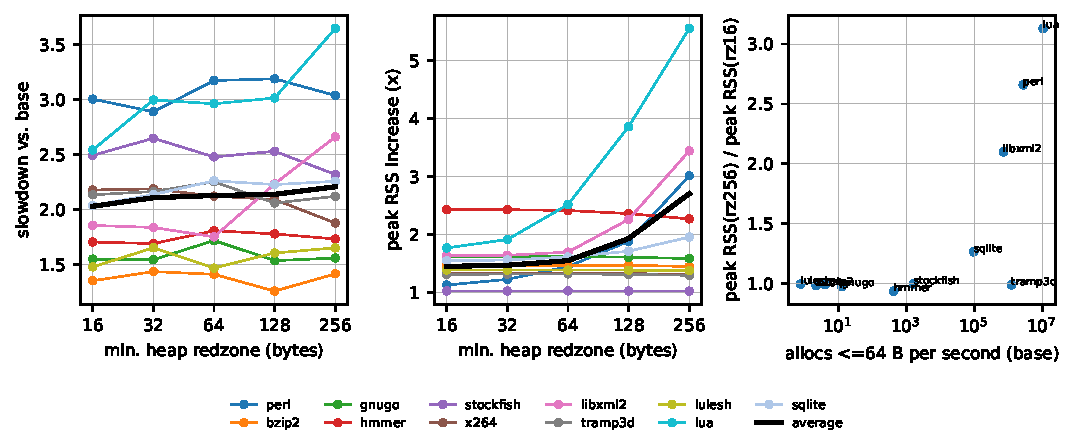
\includegraphics[width=\linewidth]{figures/fig_redzone.pdf}
\caption{Extension: minimum heap redzone vs.\ slowdown (left) and peak-RSS
increase (middle), per program and on average (black). Right: memory
sensitivity (peak RSS at 256\,B divided by that at 16\,B) vs.\ the rate of small
allocations.}\label{fig:rz}
\end{figure}

\begin{table}[h]
\centering\small
\caption{Extension: slowdown (T) and memory increase (M, peak RSS) per
minimum redzone size. Averages: mean $\pm$ s.d.\ over \RzRuns{}
repetitions (T) and ratio of totals (M).}\label{tab:rz}
\begin{tabular}{lrrrrrrrr}
\toprule
Benchmark & T rz16 & T rz32 & T rz64 & T rz128 & T rz256 & M rz16 & M rz128 & M rz256 \\
\midrule
\texttt{perl} & 3.00 & 2.89 & 3.17 & 3.19 & 3.04 & 1.13 & 1.89 & 3.01 \\
\texttt{bzip2} & 1.35 & 1.43 & 1.41 & 1.26 & 1.41 & 1.47 & 1.48 & 1.45 \\
\texttt{gnugo} & 1.55 & 1.54 & 1.72 & 1.53 & 1.56 & 1.63 & 1.61 & 1.59 \\
\texttt{hmmer} & 1.70 & 1.69 & 1.80 & 1.78 & 1.73 & 2.43 & 2.36 & 2.27 \\
\texttt{stockfish} & 2.49 & 2.65 & 2.48 & 2.53 & 2.32 & 1.03 & 1.03 & 1.03 \\
\texttt{x264} & 2.18 & 2.19 & 2.12 & 2.09 & 1.88 & 1.34 & 1.33 & 1.32 \\
\texttt{libxml2} & 1.85 & 1.83 & 1.75 & 2.23 & 2.66 & 1.64 & 2.26 & 3.44 \\
\texttt{tramp3d} & 2.13 & 2.16 & 2.25 & 2.06 & 2.12 & 1.32 & 1.32 & 1.30 \\
\texttt{lulesh} & 1.48 & 1.65 & 1.47 & 1.60 & 1.65 & 1.39 & 1.39 & 1.38 \\
\texttt{lua} & 2.54 & 2.99 & 2.96 & 3.01 & 3.65 & 1.77 & 3.86 & 5.55 \\
\texttt{sqlite} & 2.03 & 2.13 & 2.26 & 2.22 & 2.25 & 1.55 & 1.72 & 1.96 \\
\midrule
Average & 2.03$\pm$0.10 & 2.11$\pm$0.19 & 2.13$\pm$0.11 & 2.14$\pm$0.19 & 2.20$\pm$0.11 & 1.45 & 1.93 & 2.71 \\
\bottomrule
\end{tabular}

\end{table}


% ===========================================================================
\section{Conclusion}\label{sec:concl}

\paragraph{Overall verdict.}
\emph{Partially reproduced}. With today's \asan{}, the average run-time claims (C1,
C2) and the stack and binary-size claims hold for programs comparable to the
paper's, while the 3.37$\times$ memory increase does not: we measure
\OurMemTotal$\times$ in peak resident memory, and the paper's VmPeak metric no
longer applies.

\paragraph{Lessons learned.}
\begin{itemize}
\item \emph{Settings matter as much as the mechanism.} Run-time options
(quarantine, allocation stack traces, redzone size) changed our slowdown by
up to \CtrlDefDelta{} on average and our memory increase by a factor of
almost three. A reproduction has to copy these settings, not just the
compiler flag.
\item \emph{Metrics age.} VmPeak was a sensible memory metric in 2012; with
today's 20\,TB shadow reservation it measures nothing. We had to justify a
replacement (VmHWM) and record both.
\item \emph{Workload composition drives the averages.} The slowdown is
largely explained by allocation rate. Our 11-program average is
\GapRWAllRel{} above the paper's headline number, but the like-for-like
comparison with the same seven SPEC programs agrees to within
\GapRWMapRel. A headline average is only meaningful together with the
program set it was computed on.
\item \emph{Cloud VMs are noisy.} Steal time of up to \StealMaxPct\% of a run made
interleaved repetitions, medians and steal accounting necessary before any
average could be trusted.
\end{itemize}


% ===========================================================================
\section*{Contribution Statement}
Each member's commits carry their student ID and name in the message; the Git
history of the repository shows the split below.
\begin{itemize}
\item \textbf{Hua Minqi (1240030798)}: experiment environment and builds:
\cmd{Dockerfile}, \cmd{Makefile}, source download and verification
(\cmd{scripts/fetch.sh}, \cmd{scripts/sources.txt}), the per-benchmark build
scripts and the four build configurations (\cmd{config/build\_configs.sh}),
environment recording, README and third-party licences.
\item \textbf{Li Linxuan (1240022141)}: workloads and measurement: input
generator (\cmd{scripts/gen\_inputs.py}), run scripts of the 11 programs, the
measurement harness (\cmd{scripts/run\_experiments.py},
\cmd{harness/procstat.c}, \cmd{harness/malloccount.c}), the experiment matrix
(\cmd{config/experiments.json}), and running the main, control and extension
experiments (\cmd{results/raw/}).
\item \textbf{You Te (1240037846)}: analysis and report: paper reference data
(\cmd{analysis/paper\_data.py}), analysis and plotting
(\cmd{analysis/analyze.py}), discrepancy analysis, the extension design and
this report.
\end{itemize}

\section*{AI Usage Statement}
We leverage artificial intelligence to systematically organize and analyze complex project data, transforming raw datasets into structured, actionable insights. Through intelligent code parsing and algorithmic evaluation, the AI extracts core logic, identifies architectural bottlenecks, and assesses technical feasibility with high accuracy. Based on this comprehensive analysis, it autonomously generates tailored design proposals that align with project objectives, system requirements, and engineering best practices. This end-to-end workflow not only accelerates the technical assessment and architecture phases but also ensures consistency, scalability, and data-driven decision-making throughout the project development lifecycle.

\begin{thebibliography}{9}\small
\bibitem{asan} K.~Serebryany, D.~Bruening, A.~Potapenko, D.~Vyukov.
\newblock AddressSanitizer: A Fast Address Sanity Checker.
\newblock In \emph{USENIX Annual Technical Conference (ATC)}, 2012.
\bibitem{asandoc} The Clang Team. \emph{AddressSanitizer} (Clang 18 documentation).
\newblock \url{https://releases.llvm.org/18.1.0/tools/clang/docs/AddressSanitizer.html}.
\bibitem{asanflags} Google Sanitizers wiki. \emph{AddressSanitizerFlags} (run-time options).
\newblock \url{https://github.com/google/sanitizers/wiki/AddressSanitizerFlags}.
\bibitem{spec} J.~L.~Henning. SPEC CPU2006 Benchmark Descriptions.
\newblock \emph{ACM SIGARCH Computer Architecture News}, 34(4), 2006.
\bibitem{lulesh} I.~Karlin, J.~Keasler, R.~Neely. LULESH 2.0 Updates and Changes.
\newblock Technical Report LLNL-TR-641973, 2013.
\end{thebibliography}
\end{document}
